\section{Combined Learning and Control}

%Overview. Learning background.  Control background.
Our goal is to combine learning with control to tackle the complexity
and dynamics of modern mobile systems.  We use a hierarchical Bayesian
model to learn how resource allocation affects the power and
performance of an application.  This learning framework is
computationally expensive so it runs on a remote server which sends
learned models to the mobile system.  Those models are used by a
control system that dynamically tunes application resource usage to
handle system dynamics. This section provides a brief overview of the
relevant learning and control techniques used in this paper, and then
describes the interface we propose to combine them.

\subsection{Hierarchical Bayesian Learning}

\begin{figure*}

  \subfloat[]
  {
    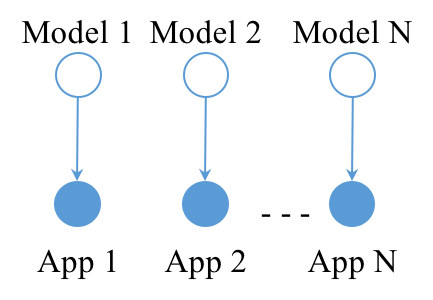
\includegraphics[width=.33\textwidth]{figs/Online.png}
    \label{fig:online}
  }
  \subfloat[]
  {
    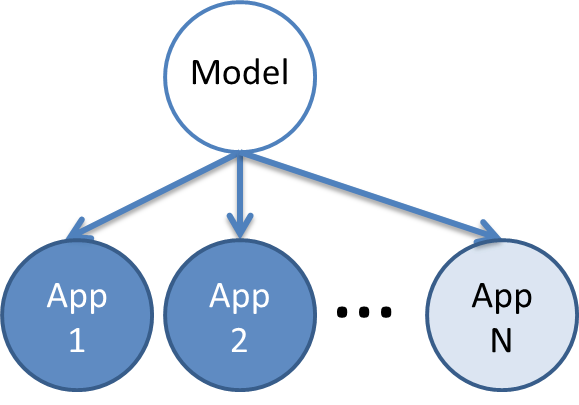
\includegraphics[width=.33\textwidth]{figs/Offline.png}
    \label{fig:offline}
  }
  \subfloat[]
  {
    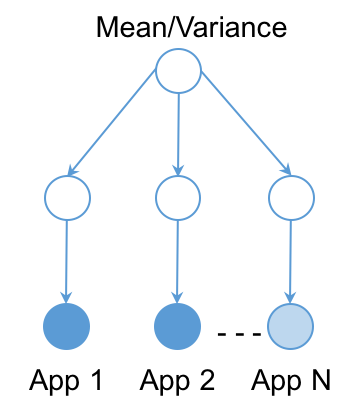
\includegraphics[width=.33\textwidth]{figs/HBM.png}
    \label{fig:HBM}
  }
  \caption{ Comparison of online (a) offline (b) and hierarchical
    Bayesian models (c).  The arrows represent dependences, circles
    are random variables, white circles are hidden variables that
    cannot be observed and must be learned, solid circles represent
    fully observed data, and shaded circles represent partially
    observed data.  The online model is concerned only with the
    current application (labeled N), the offline model combines all
    observations into one model, and the HBM builds per-application
    models, but makes them conditionally dependent on one another so
    that prior observations can be used to increase the accuracy of
    the model built for application N.}
\label{fig:learning-models}
\end{figure*}

In general, all machine learning techniques take observations of some
phenomena and turn them into a model to predict future outcomes.  In
our specific case, we want to take observations about application's
performance and power given a resource allocation and predict how
future application's will perform or how different resource
allocations will affect the current application.  

In this work, we use a hierarchical Bayesian model (HBM) to turn
observations of applications' performance and power into predictions
about how other, unobserved resource allocations will alter that
performance and power.  We use a HBM because it provides a
statistically sound framework for learning across applications and
devices.  The HBM is also well suited to learning the complicated
tradeoff spaces that arise from heterogeneity in modern mobile
processors.

When selecting a learrning framework we must find a tradeoff between
the specific and the general; \ie between frameworks that build
application-specific models and frameworks that combine observations
across applications.  For example, the key to energy efficiency on
heterogeneous mobile systems is knowing when to make use of the
smaller, low-power cores \cite{}.  An application-specific model will
capture that precisely, but may require many observations before
producing the correct model.  A more general model will capture the
trend, \eg when most applications should transition, but this general
model might miss the key inflection point for some applications.  We
refer to application-specifc models as \emph{online} because they
build models for the current application and do not incorporate
knowledge of other applicaitons.  We refer to general models as
\emph{offline} as they use prior observations of other applications to
predict the behavior of a new application.  

The HBM provides a good balance between the online and offline
approaches.  The key differences between these three approaches are
illustrated in \figref{learning-models}. In this figure, circles
represent random variables, directed edges show conditionally
dependent relationships, and shading represents observability.  A dark
circle means we have seen all the data, a shaded circle means we have
some partial observations, and the white circle means that the
variable is unobservable.  The models we are trying to learn
areunobservable.  A strictly online approach will handle each new
application completely separately and ignore observations of previous
applications.  This approach never risks contaminating a model with
unrelated observations, but it may take many observations of the
current application to converge because it starts with no prior
knowledge. The offline approach uses all observations from prior
applications and will therefore converge very quickly; however, it is
overly general and cannot learn features specific to a single
application.

The HBM (illustrated in \figref{HBM}) is a good compromise.  Each
application has its own model, allowing specificity, but these models
are conditionally dependent on some underlying probability
distribution with a hidden mean and co-variance matrix.  In practice,
the HBM will estimate a model for a new application using a small
number of observations and combining those observations with the large
number of observations previously made of similar applications.
Rather than over-generalizing, the HBM will use only similar
applications to learn models.  In addition, the HBM's accuracy
increases as more applications are observed because more different
types of behavior are represented in the pool of prior knowledge.  Of
course, the computational complexity of learning also increases with
increasing applications, but this is why we offload the learnign to a
remote server.

To provide intuition we offer a simple example.  Suppose we have
observed many prior applications, all of which are either completely
compute-bound or completely memory-bound, and we have an equal number
of both.  The only resource we can allocate is clockspeed, which will
increase the performance of compute-bound applications, but not
memory-bound ones.  When we need to work with a new application, we
need to estimate its response to clockspeed.  The online model will
not use prior knowledge, but will observe many different clockspeeds
for the new application, leading to high overhead.  The offline model
will predict the mean response of prior applications, meaning it will
overallocate speed to memory-bound applications and under-allocate to
compute-bound ones.  The HBM will take a small number of observations
and then the prediction will combine those with prior knowledge: if
the new observations show that clockspeed has no effect on performance
the HBM will use only the prior memory bound applications to build its
model, otherwise, it will use the compute-bound applications.  In
practice, the HBM can learn much more complicated tradeoffs by
combining observations of the new application with prior knowledge of
different types of behavior.

%Online Models

%Offline Models

%HBM

\subsection{Controlling COmputing SYstems}
Control theory provides a set of techniques for ensuring that a system
meets some requirement and reasoning about the ability to meet that
requirement in a dynamic environment where fluctuations cannot be
predicted ahead of time.  



\subsection{Interfacing Control and LEarning}


